\section{Proposed Architecture}

\subsection{Packet Format}:pktformat.  

There are 2 formats of data packets: data packet, and weight, bias, routing table  configuration packet. They are presented in figure~\ref{figure:pktformat}
\begin{figure}[h!]
    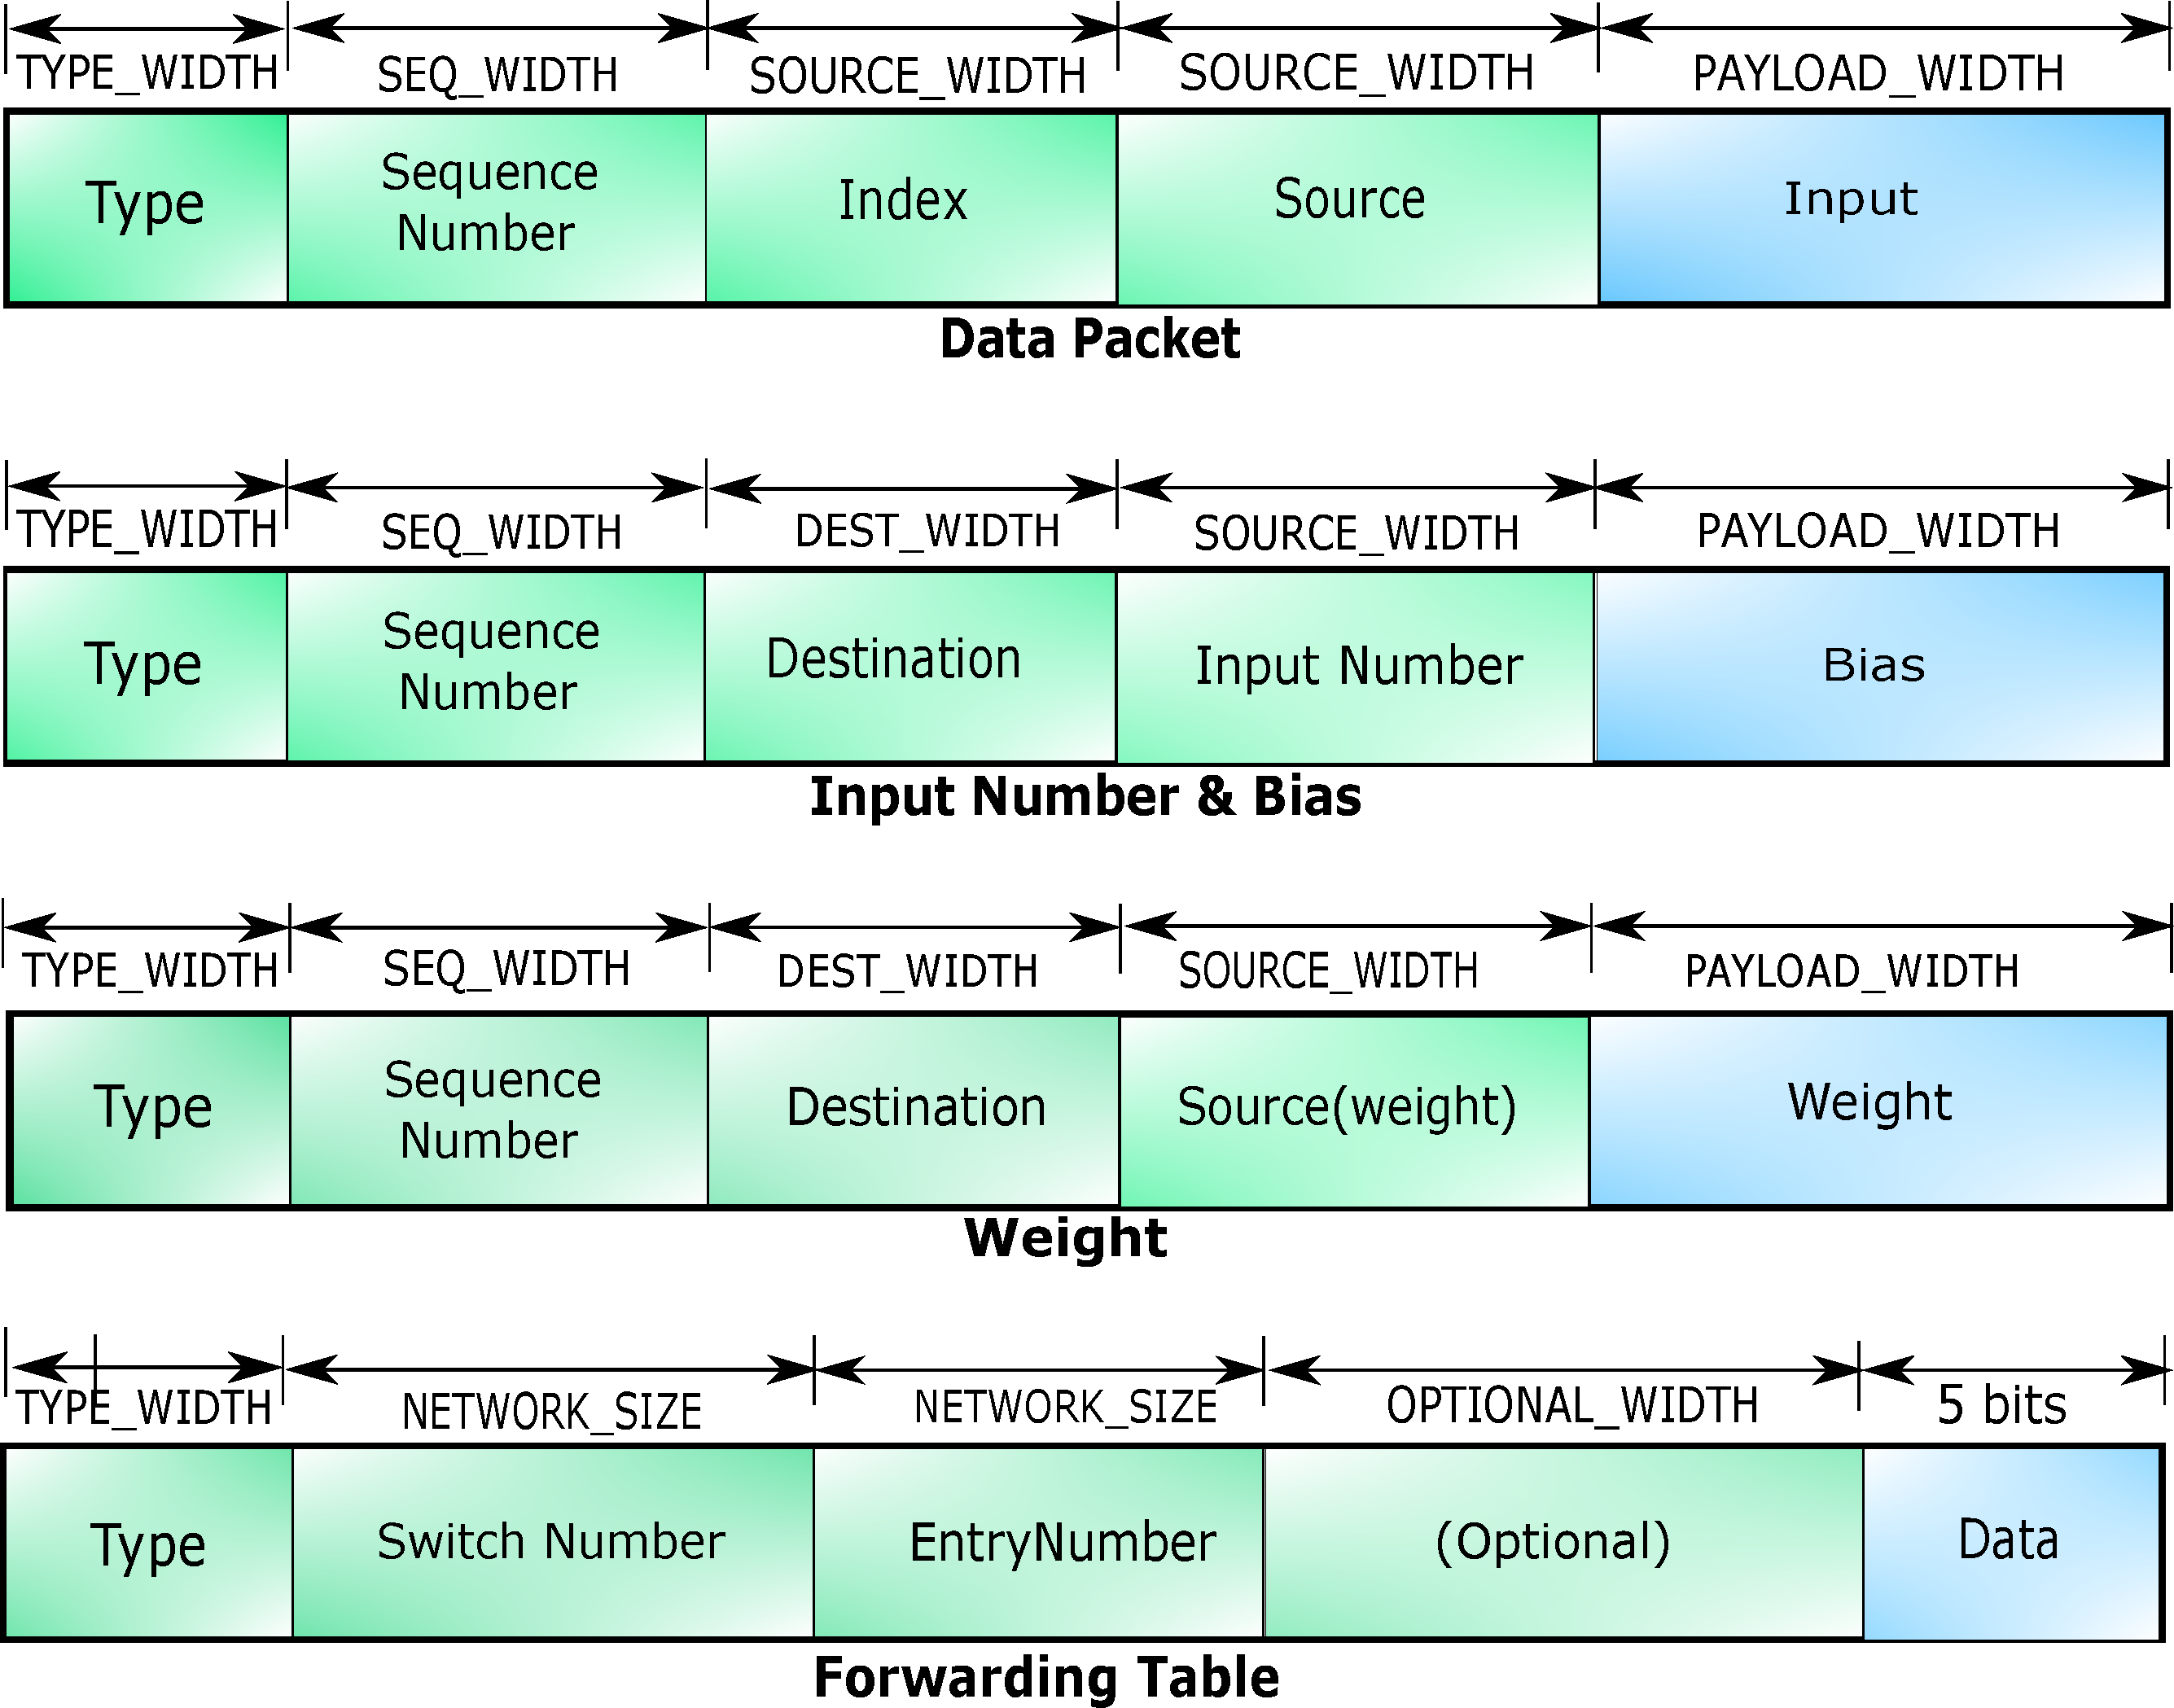
\includegraphics[width=\columnwidth]{Figures/pktformat.pdf}
    \caption{PKTFORMAT} 
    \label{figure:pktformat}
\end{figure}


\subsection{SNC}
The SNC module is a constitutive element underlying the PE design. Since the NOC network is not
designed to ensure the maintenance of correct packet ordering, an imperative design consideration is to
evade out-of-order packet delivery by storing and reassembling the incoming packets. Upon sending
input layer data, sending environment assigns each packet a sequence number which is entered into the
seqNum field. However, it is worth to note that the number being assigned corresponds to the session
number rather than to a single packet i.e a vector comprising n input layer data will be sent in n packets
with same sequence number. After processing the input data, the output packet from PE retains
sequence number of the input packets. The individual units of input layer data are differentiated using
index field, while individual hidden and output layer packets are differentiated using sourceAddress
field.

\begin{figure}
    \centering
    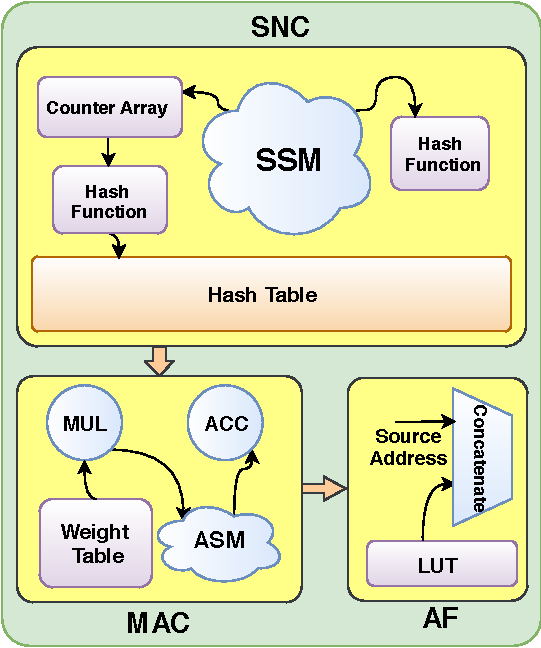
\includegraphics[width =0.4\textwidth]{Figures/overall2.pdf}
    \caption{Caption}
    \label{fig:my_label}
\end{figure}


The figure~\ref{figure:snc} depicts SNC hardware block diagram. The packets arriving from the network
interface are first stored in the hash table (HT) memory. The memory consists of $2^{SEQ\_WIDTH}$ blocks,
where $SEQ\_WIDTH$ amounts to the number of bits in the seqNum field. For the sake of full configurability, for the given NOC of size $S_{NOC}$, each PE can be configured to receive inputs
from up to $S_{NOC}$ terminals. Thus, every block is further divided to contain place for $S_{NOC}$ packets. The packets are mapped into memory through hash function, where

\begin{equation}
hf (seqNum, counter[seqNum]) = concatenate(seqNum, counter[seqNum])
\label{equation:hf}
\end{equation}

Here, the counter[seqNum] embodies the number of packets with the given sequence number that have
arrived to PE and is stored in counter array (CR). After the packet is mapped into appropriate position
within HT, the counter [seqNum] is incremented, so that the next packets with the same sequence
number is stored in the next memory location. The SNC State Machine (SSM) (figure~\ref{figure:sst})
tracks current sequence number and counter to retrieve packets from the HT. The number of inputs
linked to PE is configured using corresponding control packet.

\subsection{MAC}
The computation of the total synaptic input to the neuron constitutes the principal arithmetic operation to be implemented in a hardware design of a neural network. This is done by successive multiplication and addition operators i.e. a series of Multiply-Accumulate (MAC) operations. The reassembled packets from SNC are ushered towards Multiplication (MUL) stage. The weights are associated with the individual input packets through their source address, and these weights are stored in a Weight Table (WT) memory block which is shown in figure~\ref {figure:mac}. The weights can be configured on the run by sending corresponding control packets. The resultant product is accumulated at the Accumulation (ACC) stage. Assuming same format for neuron input and output data, the number of bits to represent weighted sum is

\begin{equation}
N_{s}=\lceil\log_{2}(S_{NOC}\cdot (2^{n_{w}-1})(2^{n_{z}-1})+2^{n_{b}-1}\cdot 2^{f_{z}+f_{w}+f_{b}})\rceil+1
\label{equation:Ns}
\end{equation}

The number of inputs and bias are configured with the same control packets which were used during SNC.  

\subsection{AF}
Implementation of a highly complicated and non-linear activation function, such as a sigmoid function, exploits look-up table (LUT), which may require large amount of memory area depending upon the desirable precision.  If we define $n_{s}$ as the most significant bits of $N_{s}$, increasing the value of $n_{s}$ contributes to the accuracy of the LUT at the expense of memory size. The minimum value at which all the possible output values are present in the LUT is given by

\begin{equation}
n_{s}=i_{s}-\lceil\log_{2}(\frac{d_{z}(1)}{{f}'(0)})\rceil
\label{equation:ns}
\end{equation}

Furthermore, if we consider sigmoid function, most of the entries located too far away from 0 are replicated. With this in mind, it is possible to reduce the size of LUT to store the central interval $[x_{high}, x_{low}]$, in where expressions for $x_{min}$ $x_{max}$ are given by

\begin{equation}
x_{high}=d_{s}(\ln{2^{f_{z}-1}}), x_{low}=-x_{high}
\label{equation:interval}
\end{equation}

and the number of bits to address the LUT is 
$n_{LUT}=\lceil\log_{2}{(x_{high}-x_{low}+1)}\rceil$.
If the computed weighted sum falls within the central interval, then the output is taken from the LUT otherwise the output is assigned either 1 or 0. 


\subsection{NoC}
The figure~\ref{figure:mesh} illustrates the architecture of neural NoC which consists two parts: switches and PE for each of them. The size of NoC can be customized varying $X\_SIZE$ and $Y\_SIZE$,  subsequently number of switches, PE and size of neural network can be configured. For NoC the mesh topology was used, since this topology is convenient for multicast data transmission. Switches connected to each other with four directions: North,South, East, West. Each switch connected to its PE and both of them has unique number depending on their location in the NoC. Each switch and corresponding PE have a unique number depending on their location in the NoC. The sequence starts from left bottom coordinate and increases from left to right and from bottom to top. 

\begin{figure}
    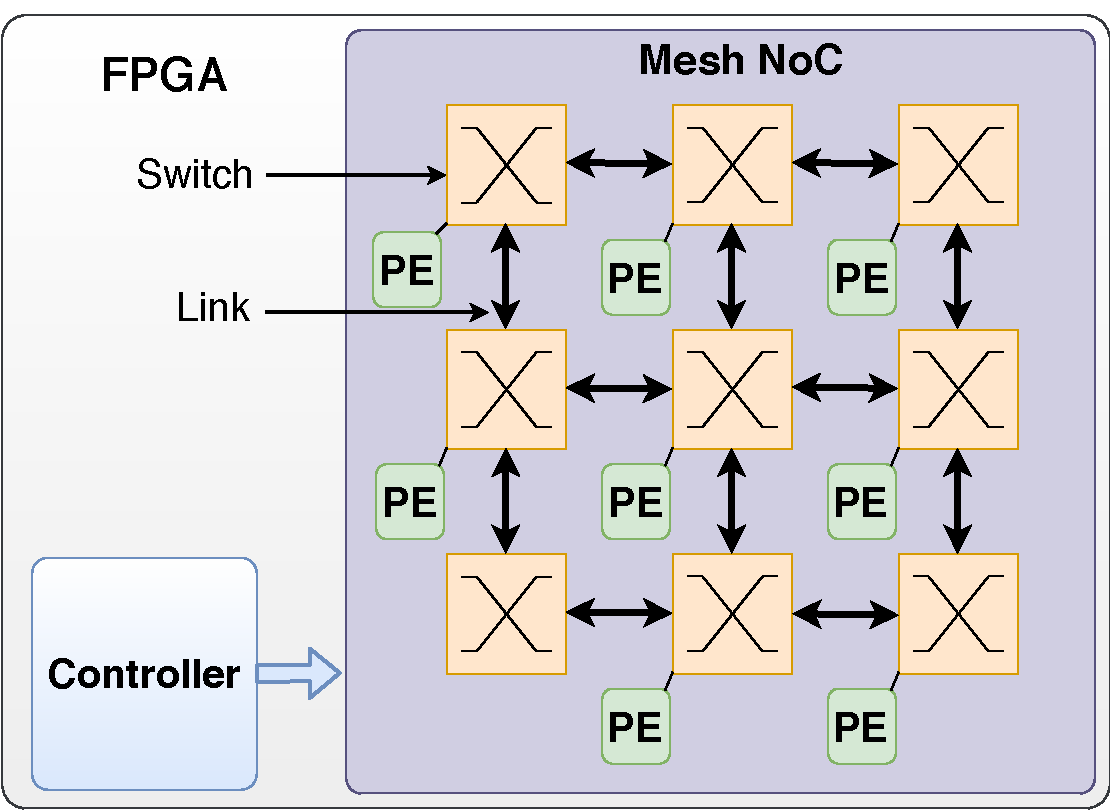
\includegraphics[width=\columnwidth]{Figures/overall3.pdf}
    \caption{MESH} 
    \label{figure:mesh}
\end{figure}

\subsection{Switch}
The inner architecture of one switch is depicted in figure ~\ref{figure:switch_architecture}. Each switch able to send and accept packets from five direction: North, South, East, West and PE. In other words, switch can communicate with upper, lower, right, left neighboring switches and with own PE. Each direction has two FIFO for receiving and transmitting the data. The FIFO was implemented by using IP FIFO generator, therefore, the depth of them can be customized. Switches serve the FIFOs in a queue in a clockwise direction.  Flow control is implemented through AXI-stream control signal as shown if figure.  The $o\_valid$ wires are asserted whenever switch transmits the data for certain direction including PE. Similarly, whenever the data comes from other switches or PE the $i\_valid$ wire of incoming side of the switch is asserted. The switch asserts the $o\_ready$ signal whenever the FIFO has empty slot to accept the data. All FIFOs should hold the data on the bus until data is transmitted to all necessary FIFO. Each switch has registers for routing table, size of total size of NoC rows with 5 bits length. Switch has finite state machine controller, which routes the packet for certain directions depending on the packet type and refreshes the routing table. In one process time one packet can be transmitted to several FIFOs. Switches communicate with each other through FIFOs.  

\begin{figure}
    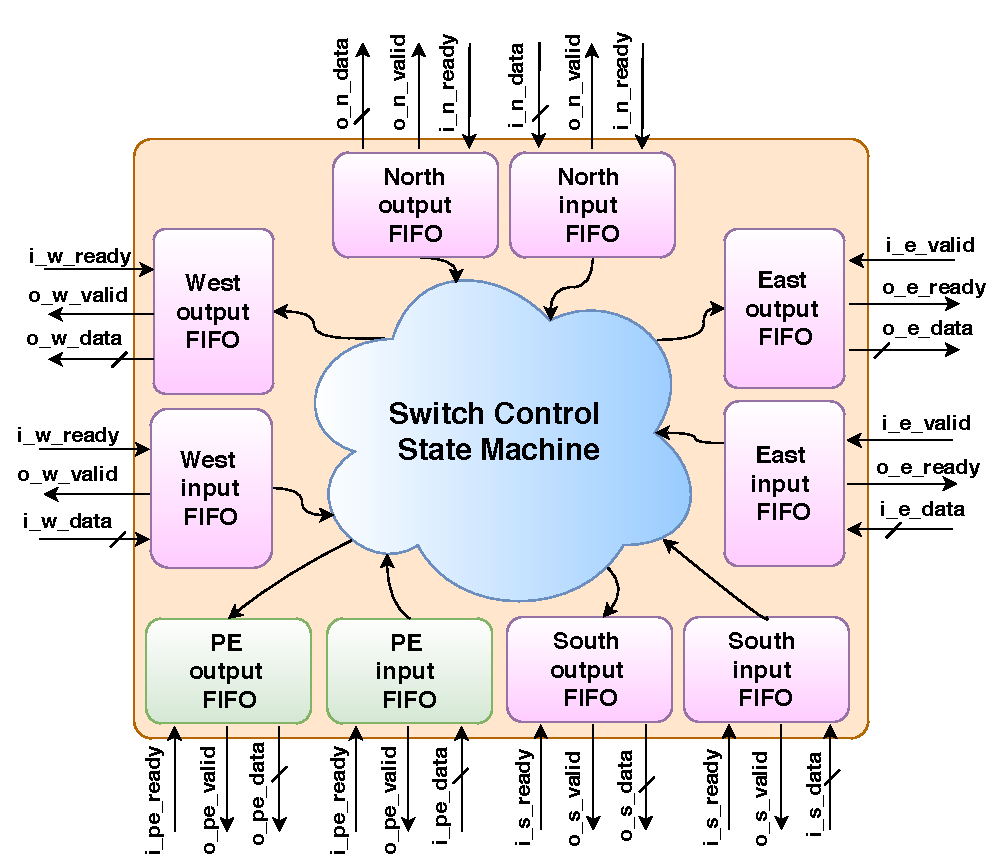
\includegraphics[width=\columnwidth]{Figures/switch2.pdf}
    \caption{Switch Architecture} 
    \label{figure:switch_architecture}
\end{figure}

\subsection{Routing Packets}
 Switch receives the packet from one FIFO and routes the data for required FIFOs. Finite state machine controller has three main approaches for routing the packets depending on the type of incoming packet.
 For weight and bias configuration packet switch sends the packet using the number of switch in the NoC. Depending on the number of destination switch, the present switch can route the packet for four directions. If the destination switch is located to the above, below, to the left or the right, it sends to North,South, East, West FIFOs respectively. Once the packet came to the predefined switch, instantly it will be sent to the PE FIFO corresponding to that switch for configuring the weight and bias.   
For routing table configuration packets switches behave the same as for weight and bias configuration oriented switches. The one difference is, when the packet came to the destination switch, it will refresh one slot of routing table and switch will serve next FIFO. 

While previous packets can be sent only for one direction(unicast) from one switch, the data packets can be replicated and sent for all direction including PE in one process time (multicast). It was achieved by the logic of routing table. Each switch has routing table, which must be configured before usage. The rows in routing table is equal to the total amount of switches in NoC. The actual meaning of rows in routing table is address of source switch. Whenever data packet comes, switch checks the source provider address of this packet and takes the row, which number is equal to source address. Each row has 5 bits for the decision to sending the packet for certain direction.  Each bit corresponds to 5 directions: North, South, East, West and PE. If the bit is equal to 1 then the incoming packet must be sent to corresponding direction,conversely, if bit is equal to 0 then the packet must not be sent to that direction. The routing table configuration directly depends on the neural network model and configuration packets must be created manually or using other software. For reliability of data in multicasted transmission, switch waits until the data is sent for all necessary direction, only after that it checks next FIFO. For implementation of packet routing the finite state machine principle was used and it is shown in figure ~\ref{figure:fsm}.


